\clearpage\begingroup\NoSourceHead\SourceLeaf{495b}
\makeatletter\tagsleft@true\let\veqno\@@leqno\makeatother
\renewcommand{\thefootnote}{\arabic{footnote})}\setcounter{footnote}{53}
\newcommand{\BolzaEqualAboveGreater}{\mathrel{\vcenter{\hbox{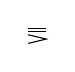
\begin{tikzpicture}[x=1em,y=1ex,line width=.04em]
\draw(0,.95)--(.65,.95);\draw(0,.70)--(.65,.70);\draw(0,.40)--(.65,.04)--(0,-.32);
\end{tikzpicture}}}}}
\ArithmeticHead{38}{L}{BOLZA, GAUSS UND DIE VARIATIONSRECHNUNG.}
\noindent\hspace*{\parindent}20. Mit der Herleitung der Randbedingung für das spezielle \textsc{Gauss}sche
Variationsproblem war im wesentlichen zugleich auch die allgemeine Aufgabe
gelöst, für das Extremum eines Doppelintegrals von der Form
\begin{equation*}
J=\iint V(x,y,z,p,q)\,dx\,dy\tag{53}
\end{equation*}
die Randbedingung aufzustellen, wenn die Begrenzungskurven der zulässigen
Flächen auf einer gegebenen Fläche
\begin{equation*}
z=g(x,y)\tag{54}
\end{equation*}
liegen sollen. Denn die Verbindung der \textsc{Lagrange}schen Formel (22) mit dem
\textsc{Gauss}schen Fundamentalsatz (41) liefert, wenn die \textsc{Lagrange}sche partielle
Differentialgleichung erfüllt ist, die »Grenzgleichung«
\begin{equation*}
\int[(Py'-Qx')(\delta z-p\delta x-q\delta y)+V(y'\delta x-x'\delta y)]\,dt=0,\tag{55}
\end{equation*}
\clearpage\SourceLeaf{496}
\ArithmeticHead{39}{R}{GAUSS’ PRINCIPIA GENERALIA THEORIAE FIGURAE FLUIDORUM.}
\noindent wobei das Linienintegral über die Begrenzungskurve $P$ des gesuchten Flächenstücks
zu erstrecken ist, und die Variable $t$ und die Ableitungen $x',y'$ dieselbe
Bedeutung haben wie in Nr. 16. Es blieb also nur noch übrig, aus der
Gleichung (55) die letzten Folgerungen zu ziehen. Hierüber soll noch kurz
berichtet werden.

Die Gleichung (55) findet sich zuerst (1831) bei \textsc{Bordoni}\footnote{\textsc{Bordoni}, loc. cit. 37), Art. 424.}, allerdings in
Folge des in Nr. 16 erwähnten Vorzeichenfehlers mit verkehrtem Vorzeichen
vor den mit $x'$ multiplizierten Gliedern. Um von hier aus zur Randbedingung
zu kommen, drückt \textsc{Bordoni} mittels der aus (54) durch Variation folgenden
Gleichung
\begin{equation*}
\delta z=g_x\delta x+g_y\delta y\tag{56}
\end{equation*}
$\delta z$ durch $\delta x$ und $\delta y$ aus und schliesst dann, dass die Koeffizienten der willkürlich
bleibenden Variationen $\delta x$ und $\delta y$ verschwinden müssen. Das ergibt
die beiden Gleichungen
\begin{equation*}
\left\{\begin{aligned}
\mp(g_x-p)Qx'+((g_x-p)P+V)y'&=0,\\
\mp((g_y-q)Q+V)x'+(g_y-q)Py'&=0.
\end{aligned}\right.\tag{57}
\end{equation*}
Darin ist das obere Zeichen das richtige, das untere das \textsc{Bordoni}sche. Hieraus
folgert \textsc{Bordoni} durch Elimination von $x',y'$ die Gleichung
\begin{equation*}
(g_x-p)P+(g_y-q)Q+V=0.\tag{58}
\end{equation*}

Dies ist in der Tat die richtige Randbedingung, und \textsc{Bordoni} gebührt
das Verdienst, sie zum ersten Mal aufgestellt zu haben; auch hat er sie
zuerst auf den speziellen Fall der Minimalflächen angewandt. Aber er hat
dieses Resultat nur dadurch erreicht, dass er zu dem ersten Fehler noch einen
zweiten hinzufügt: Die Eliminante zwischen den beiden Gleichungen (57) lautet
nämlich sowohl bei den richtigen wie bei den falschen Vorzeichen
\[
V[(g_x-p)P+(g_y-q)Q+V]=0,
\]
und \textsc{Bordoni} setzt ganz willkürlich den zweiten Faktor gleich null, während
er, wie wir sehen werden, den ersten hätte gleich null setzen müssen.

Zu den beiden Gleichungen (57) tritt nämlich noch eine dritte hinzu.
\clearpage\SourceLeaf{497}
\ArithmeticHead{40}{L}{BOLZA, GAUSS UND DIE VARIATIONSRECHNUNG.}
\noindent Denn aus der entlang der Begrenzung $P$ geltenden Gleichung $z(x,y)=g(x,y)$
folgt durch Differentiation nach $t$ die folgende zuerst von \textsc{Poisson}\footnote{\textsc{Poisson}, loc. cit. 30), S. 314.} herangezogene
Gleichung
\begin{equation*}
(g_x-p)x'+(g_y-q)y'=0.\tag{59}
\end{equation*}
Durch Elimination von $x',y'$ aus den drei Gleichungen (57) und (59) folgen
aber bei den \textsc{Bordoni}schen Vorzeichen im Allgemeinen zwei von einander
unabhängige Randbedingungen, nämlich
\[
V=0,\quad(g_x-p)P-(g_y-q)Q=0,
\]
also ein falsches Resultat, wie es bei dem falschen Ausgangspunkt zu erwarten
war. Dagegen ergibt dieselbe Elimination bei den richtigen Vorzeichen nur
die \textls[100]{eine} Bedingung (58). Es ist jedoch einfacher, wie dies \textsc{Poisson} tatsächlich
tut, die Gleichung (59) unmittelbar zur Umformung des Linienintegrals (55)
zu benützen, nachdem man darin $\delta z$ durch $\delta x$ und $\delta y$ ausgedrückt hat. Man
erhält so
\[
\int[P(g_x-p)+Q(g_y-q)+V](y'\delta x-x'\delta y)\,dt=0,
\]
woraus unmittelbar die Gleichung (58) folgt. In der Tat hat \textsc{Poisson} die allgemeine
Randbedingung (58) zuerst richtig \textls[100]{bewiesen}\footnote{Allerdings steht die Randbedingung (58) in dieser Form nicht bei \textsc{Poisson}, vielmehr ist sie als
spezieller Fall in dem entsprechenden Resultat für den allgemeineren, von \textsc{Poisson} behandelten Fall enthalten,
wo unter dem Doppelintegral auch die zweiten Ableitungen $r,s,t$ von $z$ vorkommen, und die auf
diesen allgemeinen Fall bezüglichen Formeln von \textsc{Poisson} enthalten einen schon von E. G. \textsc{Björling} bemerkten
und verbesserten Rechenfehler (\textit{Calculi variationum integralium duplicium exercitationes}, Upsala 1842); die
richtigen Formeln gibt auch \textsc{Todhunter}, loc. cit. 5), S. 85, 86.}.

21. Fragen wir schliesslich noch, welche \textls[100]{Einwände} sich etwa vom
Standpunkt der modernen kritischen Variationsrechnung aus gegen die \textsc{Gauss}sche
Schlussweise erheben lassen, so ist zunächst hervorzuheben, dass \textsc{Gauss}
von der \textsc{Euler}schen Auffassung des Variationsprozesses als Differentiation nach
einem Parameter keinen Gebrauch macht; und doch hat erst diese Auffassung
die Variationsrechnung auf eine feste Grundlage gestellt. Denn erst die Betrachtung
von ein- (oder mehr-) parametrigen Scharen von zulässigen Variationen
ermöglicht es, aus dem Vorzeichen der ersten Variation einen strengen
Schluss auf das Vorzeichen der vollständigen Variation zu machen und so die
\clearpage\SourceLeaf{498}
\ArithmeticHead{41}{R}{GAUSS’ PRINCIPIA GENERALIA THEORIAE FIGURAE FLUIDORUM.}
\noindent Notwendigkeit des Verschwindens der ersten Variation zu beweisen. In der
Tat hat denn auch \textsc{Lagrange} in seinen späteren didaktischen Schriften über
Variationsrechnung\footnote{\textsc{Lagrange}, \textit{Théorie des fonctions analytiques}, Oeuvres, Bd. IX, S. 298; \textit{Leçons sur le calcul des
fonctions}, Oeuvres, Bd. X, S. 400.} diese \textsc{Euler}sche Methode seinen Entwicklungen zugrunde
gelegt. Statt dessen geht \textsc{Gauss} auf den Standpunkt von \textsc{Lagrange} und \textsc{Euler}
vor der grundlegenden Arbeit von \textsc{Euler}\footnote{\textsc{Euler}, loc. cit. 3).} vom Jahr 1771 zurück.

Damit hängt auch die Tatsache zusammen, dass \textsc{Gauss} nicht ausdrücklich
zwischen \textls[100]{vollständiger} Variation und \textls[100]{erster} Variation unterscheidet. Die
Variationen $\delta x$, $\delta y$, $\delta z$ sind ihm willkürliche »unendlich kleine« Funktionen
von $x$, $y$, und die Grössen $\delta W$, $\delta s$, die tatsächlich erste Variationen sind,
werden so behandelt, als ob sie vollständige Variationen wären. So schliesst
er: Für ein Minimum muss $\delta W\BolzaEqualAboveGreater0$ sein für alle unendlichkleinen mit der
Gestalt des Gefässes vereinbaren Formveränderungen der Flüssigkeit, für
die $\delta s=0$. Das ist ohne weiteres klar für die \textls[100]{vollständigen} Variationen,
nicht aber für die \textls[100]{ersten} Variationen. Hier liegt in der Tat eine fundamentale
Lücke vor, die sich durch die ganze vor\textsc{weierstrass}sche Variationsrechnung
hindurchzieht. Geht man nämlich von der Betrachtung einer Schar
zulässiger Flächen
\begin{equation*}
\bar x=X(x,y,\varepsilon),\quad\bar y=Y(x,y,\varepsilon),\quad\bar z=Z(x,y,\varepsilon)\tag{60}
\end{equation*}
aus und definiert
\begin{equation*}
\delta x=\varepsilon X_{\varepsilon}(x,y,0),\quad
\delta y=\varepsilon Y_{\varepsilon}(x,y,0),\quad
\delta z=\varepsilon Z_{\varepsilon}(x,y,0),\tag{61}
\end{equation*}
so genügen die Funktionen $\delta x,\delta y,\delta z$ der Gleichung
\begin{equation*}
\left\{\begin{gathered}
\delta s=0\\
\text{und überdies entlang der Begrenzung der Gleichung}\\
\delta z=g_x\delta x+g_y\delta y.
\end{gathered}\right.\tag{62}
\end{equation*}

Der Schluss, dass
\[
\delta W\BolzaEqualAboveGreater0
\]
sein muss für alle Funktionen $\delta x,\delta y,\delta z$, die den Gleichungen (62) genügen,
\par\smallskip\noindent{\small X$_2$ Abh. 5.}\hfill{\small 6}\par
\clearpage\SourceLeaf{499}
\ArithmeticHead{42}{L}{BOLZA, GAUSS UND DIE VARIATIONSRECHNUNG.}
\noindent ist aber erst berechtigt, nachdem gezeigt ist, dass man zu jedem Funktionensystem
$\delta x,\delta y,\delta z$, das den Gleichungen (62) genügt, eine Schar zulässiger
Flächen (60) konstruieren kann, für welche die Gleichungen (61) bestehen.

Die Erkenntnis, dass die Betrachtung der ersten Variationen nicht ausreicht,
dass es vielmehr nötig ist, von den ersten Variationen zu den vollständigen
Variationen aufzusteigen, verdankt man \textsc{Weierstrass}, und seitdem
bildet die Herstellung von Scharen zulässiger Variationen bei allen strengen
Beweisen, die sich auf Variationsprobleme mit Nebenbedingungen (Grenzbedingungen
einbegriffen) beziehen, einen wesentlichen Teil der Untersuchung.
Von alledem findet sich bei \textsc{Gauss} noch nichts.
\par\clearpage\endgroup
